%------------------ About -----------------------
% McMaster Master's/Doctoral Thesis
% LaTeX Template, Version 1.1 (07 Aug 2022)
% Works for only Double Spaced Thesis
% Compiler: pdfLaTeX
% TeX Live version: 2020 (Legacy)

% First modifications according to McMaster SGS 2016 Guideline:
% Dr. Omar Boursalie
%
% Updated according to McMaster SGS 2021 Guideline and made compatible to Overleaf:
% Asif Khan (https://www.linkedin.com/in/asif-k/)
% will occasionally update on Overleaf template page
%
% Thanks to Sajjad Rashidiani for help in rechecking

%---------------- V1.1 --------------------------
% matched updated style format for double spacing by Mac SGS guideline (Aug 2021)
% Removed manual packages (in backup: fancyheadings, natbib) and added packages in preamble to work well in Overleaf
% Organized files, folders and renamed a few to match overall format
% Added hyperlinks and made it dynamic
% Other minor changes

% License:
% CC BY-NC-SA 4.0 (https://creativecommons.org/licenses/by-nc-sa/4.0/)

%----------------- preamble ------------------
\documentclass[letterpaper, 12pt]{report}                  % Letter paper, Times New Roman, 12pt, twoside or oneside

% new packages
\usepackage{lipsum}
\usepackage[utf8]{inputenc}
\usepackage{comment}
\renewcommand{\contentsname}{Table of Contents} % to rename it from Contents to Table of Contents % https://tex.stackexchange.com/questions/28516/how-to-change-the-title-of-toc
\usepackage[backend=biber,style=numeric-comp]{biblatex} % Bibliography formatting
\addbibresource{../refs/References.bib}
\usepackage{fancyhdr}                           % Header and footer styling

\usepackage{gscale_thesis_doublespace}          % Double spaced thesis

\usepackage{setspace}    % Allows double spacing but skips headers/footers
% all the definitions are here

% thesis information
\halftitle{Exploring a GMRES Solver Implementation} % 60 Characters Max. Including Spaces
\title{Exploring Sparse Linear Solver Implementations: GMRES with Iterative Refinement and Fine-Grained Parallel ILU in Mixed Precisions}
\field{Scientific Computing} % What field your thesis is in (if needed)

% your information
\author{Xunzhou Ye}
\shortauthor{X. Ye} % Used for page header

% school information
\dept{\href{https://www.eng.mcmaster.ca/cas}{Computing \& Software}} % Your department's name, print it using \@dept
\gschoolname{\href{https://gs.mcmaster.ca/}{School of Graduate Studies}}
\univname{\href{http://www.mcmaster.ca/}{McMaster University}} % Your university's name, print it using \@univname
\macaddress{Hamilton, Ontario, Canada}

% previous and current degrees
\prevdegreeone{BEng (Software Engineering),\\ McMaster University, Hamilton, Canada}
\prevdegreetwo{BEng} % Just your degree's field
\degreename{Master of Engineering}

% date and time
\submitmonthyear{September 2025} % did not make dynamic on purpose
\submitdate{\today} % please use with caution
\copyrightyear{2025} % did not make dynamic on purpose

% Supervisor/Committee
\principaladviser{Dr. Ned Nedialkov} % Your Supervisor
    % LaTeX variables for preface pages/headers
\setcounter{tocdepth}{1} % Limits the TOC to chapter and section names

% Additional packages
\usepackage{graphicx}                         % Allows the inclusion of figures
\usepackage{subcaption}                       % Allows captions to be added to subfigures
% \usepackage[justification=centering]{caption} % Centres caption text
\usepackage{caption}                          % Caption text
\usepackage[hidelinks]{hyperref}              % Linking to LaTeX labels and external URLs
\usepackage{array}                            % Used for table formatting
\newcolumntype{P}[1]{>{\raggedright\let\newline \\\arraybackslash\hspace{0pt}}m{#1}}
\usepackage{booktabs}                         % Fancy-style tables
\usepackage{longtable}                        % Allows for tables that are more than one page long
\usepackage{float}                            % Better figure placement control
\usepackage{enumerate}
\usepackage[shortlabels]{enumitem}            % Numbered lists
\usepackage[shortcuts]{extdash}               % Allows manual hyphenation of hypenated words
\usepackage{amsmath}                          % Non-standard math symbols
\usepackage{amssymb}
\usepackage{amsfonts}                         % Extended fonts for mathematics
\usepackage{mathtools}
\numberwithin{equation}{section}              % Numbers equations based on their section
\usepackage{tikz}
\usepackage{listings}
\usepackage{algpseudocode,algorithm}
\usepackage{threeparttable}
\usepackage{siunitx}
\sisetup{exponent-product = \cdot}
\sisetup{print-zero-exponent = true}
\sisetup{tight-spacing = true}

\DeclareMathOperator{\ILU}{ILU}
\DeclareMathOperator*{\argmax}{arg\,max}
\DeclareMathOperator*{\argmin}{arg\,min}

%----------------- Document Begins ------------------
\begin{document}

% --------------------Before Preface-------------------------
\beforepreface                                       % Half title page, title page, declaration page
% \include{chapters_before_preface/1_lay_abstract}     % Lay Abstract
\prefacesection{Abstract}

This work presents the design and implementation of a mixed-precision iterative
refinement (IR) solver for large sparse linear systems, combining fine-grained
parallel incomplete LU (ILU) preconditioning with GMRES. The solver is
implemented in modern C++ with extensive use of templates and concepts to
enforce precision hierarchies, providing flexibility to employ IEEE 754 and
extended floating-point formats. To support extended precision, functionality
was added to the QD library. A modular BLAS-like kernel layer decouples
low-level operations from solver logic, enabling mixed-precision operations
across factorization, Krylov iterations, and residual computations.

Experimental evaluation across a set of sparse matrices highlights the accuracy
and performance trade-offs of mixed-precision configurations. Results show that
increasing factorization precision accelerates convergence, while higher
residual precision stabilizes residual computation without significantly
reducing iteration counts. However, the overall performance is dominated by the
GMRES solve phase, limiting the observed gains from reduced-precision
factorization. The study concludes that while mixed-precision arithmetic offers
potential runtime advantages, the benefits in the current GMRES-IR pipeline
remain modest.
         % Abstract
% \include{chapters_before_preface/3_dedication}       % Dedication
\prefacesection{Acknowledgements}

I would like to express my sincere gratitude to my supervisor, Dr. Ned
Nedialkov, for his guidance, patience, and invaluable feedback throughout the
course of this work. I am also thankful to the teaching and research staff of
the Department of Computing \& Software, whose support and resources made this
project possible.
 % Acknowledgements
\referencepageswithnotations{notation}               % Table of Contents, List of Figures, List of Tables, Notations
% \referencepages % No notations version (choose one)???
\prefacesection{Declaration of Academic Achievement}

I, Xunzhou Ye, hereby declare that this report is the result of my own work and
has not been submitted, either in whole or in part, for the award of a degree at
this or any other institution. All sources of information and contributions from
others have been properly acknowledged and cited.
  % declaration of Academic Achievement

% add your new chapters here according to your text file name
% --------------------After Preface-------------------------
\afterpreface
\chapter{Introduction}
\label{cha:introduction}

In numerical computing, solving large sparse systems of linear equations
efficiently and accurately is a fundamental challenge with wide applications in
scientific computing, optimization, and engineering simulations. Traditional
double precision direct solvers, though robust, often suffer from high memory
demands and computational cost, particularly due to fill-in during factorization
of sparse matrices. This has motivated the development of iterative methods and
preconditioning strategies that aim to balance efficiency and accuracy.
Concretely, we are concerned with solving linear systems of the form \[\matr{A}
  \vec{x} = \vec{b}, \] where \(\matr{A} \in \mathbb{R}^{n \times n}\) is a
symmetric, nonsingular, sparse matrix and \(\vec{b} \in \mathbb{R}^n\) is a
specified right-hand side vector.

One promising approach is mixed-precision iterative refinement (IR), which
leverages lower precision arithmetic for speed while retaining high precision
steps to ensure stability and accuracy. In particular, the GMRES-based iterative
refinement (GMRES-IR) method combines iterative refinement with the Generalized
Minimal Residual method (GMRES), enabling robust convergence even for
ill-conditioned systems \cite{lindquist_improving_2020,mary_mixed_2023}.
Mixed-precision algorithms have been shown to significantly reduce the
time-to-solution by exploiting modern hardware accelerators and memory
hierarchies, while maintaining accuracy comparable to traditional
double-precision solvers \cite{mary_mixed_2023}.

This project builds on prior work by \textcite{wong_exploring_2024}, who developed
a prototype GMRES-IR solver with theoretical analysis in a five-precision
setting. Building on this foundation, the present work explores and experiments
with a practical implementation of GMRES-IR in C++, emphasizing both algorithmic
advances and software design improvements. The solver supports mixed precision
across different stages of the refinement process, enforced through C++
templates and concepts that explicitly separate factorization, working, and
residual precisions. Compared to the earlier implementation, the codebase has
been modernized with a cleaner interface, integrated CMake build integration,
and improved modularity.

A key obstacle in earlier GMRES-IR implementations was the reliance on
LDL\textsuperscript{T} factorization (via a modified QDLDL package
\cite{shahrooz_derakhshan_using_2023}) for preconditioning, which incurred
substantial fill-in and dominated the runtime. To address this, we replace
LDL\textsuperscript{T} with a fine-grained parallel incomplete LU (ILU)
factorization \cite{chow_fine-grained_2015}, which provides a less accurate but
effective preconditioner with significantly reduced memory overhead.
Implementing ILU in parallel within a mixed-precision framework requires careful
design but enables scalability to much larger sparse problems. In the present
implementation, ILU is applied only to symmetric matrices. Most of these are
symmetric positive definite (SPD), though some are indefinite. While ILU is, in
principle, applicable to general nonsymmetric systems, robust application in
that setting typically requires reordering or pivoting to ensure stability,
which is beyond the scope of this project. Restricting attention to symmetric
(mostly SPD) matrices keeps the implementation tractable while still allowing
evaluation of the effectiveness of a mixed-precision GMRES-IR solver with
parallel ILU preconditioning.

The main contribution of this report is an experimental study of the performance
trade-offs in mixed-precision GMRES-IR with parallel ILU preconditioning. We
investigate the effects of precision choice, Krylov subspace size, and
preconditioning quality on both runtime and accuracy when solving large sparse
systems. While the implementation is not yet a polished solver intended for
production use, it provides insight into practical aspects of mixed-precision
iterative refinement and contributes to the broader goal of developing robust,
efficient open-source solvers.

The remainder of this report is structured as follows:

\begin{itemize}
\item Chapter \ref{cha:literature-review} reviews the relevant literature, covering
  the foundations of iterative solvers, preconditioning techniques, and
  mixed-precision computing.
\item Chapter \ref{cha:math-form} presents the mathematical formulation of the core
  algorithms, including the GMRES method, the iterative refinement framework,
  and the fine-grained parallel ILU factorization.
\item The C++ implementation of the solver is described in Chapter
  \ref{cha:implementation}, with a focus on its software architecture, use of
  templates to ensure precision flexibility, and modular design.
\item In Chapter \ref{cha:exper-eval}, we present a comprehensive experimental
  evaluation, assessing the solver’s accuracy and performance across a benchmark
  of sparse matrices and analyzing the trade-offs of various mixed-precision
  configurations.
\item Finally, Chapter \ref{cha:conclusion} concludes the report with a summary of our
  findings and offers directions for future research.
\end{itemize}

\setcounter{figure}{0}
\setcounter{equation}{0}
\setcounter{table}{0}

\chapter{Literature Review}
\label{cha:literature-review}

This chapter provides an overview of existing research and foundational concepts
relevant to improving the performance of the GMRES method using mixed-precision
techniques. It covers iterative solvers in the context of mixed-precision
computing and several preconditioning strategies.

\section{Iterative Solvers and MP Computing}
\label{sec:iterative-solvers}

The Generalized Minimum Residual (GMRES) method, introduced by
\citeauthor{saad_gmres_1986} in \citeyear{saad_gmres_1986}, is a widely used
iterative, Krylov subspace method for solving sparse, non-symmetric systems of
linear equations arising from many scientific applications
\cite{saad_gmres_1986}. As a Krylov subspace method, GMRES constructs an
orthogonal basis using Arnoldi’s procedure and then finds a solution vector
within that subspace such that the resulting residual is minimized.

A significant extension to GMRES is the introduction of restarting, where the
solver computes the current solution vector after a certain number of iterations
and then restarts with an empty Krylov subspace, using the newly computed
solution as the new initial guess \cite{lindquist_improving_2020}. This
technique is vital for limiting the number of basis vectors required for the
Krylov subspace, thereby reducing storage and computation costs associated with
orthogonalizing new vectors. It is important to note that restarted GMRES can be
seen as equivalent to iterative refinement where a non-restarted GMRES computes
the error correction \cite{lindquist_improving_2020,mary_mixed_2023}.

Iterative refinement (IR) is an established technique designed to improve the
accuracy of a computed solution to a linear system by iteratively computing and
correcting errors based on the system's residuals.
\textcite{moler_iterative_1967} advanced the understanding of IR in the context
of floating-point arithmetic. \citeauthor{moler_iterative_1967} highlighted that
iterative refinement is effective in reducing roundoff errors and noted that
only one step in the process, computing the residuals, requires higher precision
arithmetic to achieve accurate final results.

Another major advancement in IR came with the adoption of mixed-precision (MP)
arithmetic. This approach typically involves performing computationally
intensive tasks, such as matrix factorization, in lower precision to gain speed
and memory efficiency, while accuracy-critical operations, like residual
computation and solution updates, are carried out in higher precision to
maintain overall numerical stability and accuracy. As reported by
\textcite{wong_exploring_2024}, early applications of MP IR utilized
single-precision for LU factorization and double precision for residual and
correction updates, improving computational efficiency while preserving
numerical stability. This concept was then extended to preconditioned GMRES
within the MP iterative refinement framework, where correction updates are
computed using the GMRES method and done in double precision.
\textcite{lindquist_improving_2020} have proven that this approach is
particularly effective for ill-conditioned linear systems.

\section{Preconditioning}
\label{sec:preconditioning}

Preconditioning is a technique used to improve the convergence behavior of
iterative linear system solvers. It works by transforming the original linear
system into an equivalent one that has a more favorable spectrum—--typically a
smaller spectral condition number or eigenvalues clustered closer to 1
\cite[p.~187]{ascher_first_2011}. The preconditioning matrix, \(\matr{M}\),
serves as an approximation to the original matrix \(\matr{A}\). Common
preconditioning strategies include left preconditioning (\(\matr{M}^{-1}
\matr{A} \vec{x} = \matr{M}^{-1} \vec{b}\)) and right preconditioning (\(\matr{A}
\matr{M}^{-1} \vec{y} = \vec{b}, \vec{x} = \matr{M}^{-1} \vec{y}\)).

Standard preconditioners include LU factorization (\(\matr{A} = \matr{L}
\matr{U}\)). A similar concept for symmetric positive definite (SPD) matrices is
Cholesky factorization (\(\matr{A} = \matr{U} \matr{U}\transpose{}\) or
\(\matr{A} = \matr{L} \matr{D} \matr{L}\transpose{}\)). The QDLDL package
modified by \textcite{shahrooz_derakhshan_using_2023} provides an \(\matr{L}
\matr{D} \matr{L}\transpose{}\) factorization routine with MP support for
quasi-definite matrices. These are symmetric matrices of a specific block form
guaranteed to have an \(\matr{L} \matr{D} \matr{L}\transpose{}\) factorization.
\textcite{wong_exploring_2024}'s work establishes a concrete C++ implementation
of a preconditioned GMRES-IR solver that supports MP arithmetic. This solver
leverages the QDLDL package for computing the \(\matr{L} \matr{D}
\matr{L}\transpose{}\) factorization of quasi-definite matrices as the
preconditioners.

However, in the context of solving large sparse linear systems, direct methods
such as LU factorization often suffer from substantial fill-in, making them
computationally expensive both in terms of memory and time. This is evident in
\cite{wong_exploring_2024} that factorization time is a dominant component of
the total runtime for large sparse matrices where \(\matr{L} \matr{D}
\matr{L}\transpose{}\) factorization is used. Since preconditioning does not
require an exact factorization but only an approximation that accelerates
convergence, incomplete factorizations such as incomplete LU (ILU) (\(\matr{A}
\approx \tilde{\matr{L}} \tilde{\matr{U}}\)) and incomplete Cholesky (IC)
(\(\matr{A} \approx \tilde{\matr{U}} \tilde{\matr{U}}\transpose\)) are commonly
employed. A fine-grained parallel ILU algorithm, proposed by
\textcite{chow_fine-grained_2015}, offers a distinct approach to computing ILU
factorizations in parallel. Their method reformulates ILU factorization as the
solution of a system of bilinear equations \((\matr{L} \matr{U})_{i,j} =
a_{i,j}\) for entries in a specified sparsity pattern. This system of unknowns
can then be solved in parallel using fixed-point iteration sweeps, where each
component of the new iterate can be computed asynchronously, often implemented
with OpenMP. A symmetric variant is available for IC factorization. A key
finding is that very few sweeps are needed to construct an effective
preconditioner.

% This fine-grained parallel approach for ILU factorization is utilized in this
% project for computing the incomplete factorizations employed as preconditioners.


\setcounter{figure}{0}
\setcounter{equation}{0}
\setcounter{table}{0}

\chapter{Mathematical Formulation}
\label{cha:math-form}

This chapter presents the mathematical foundations underlying the solver
developed in this work. We begin with a detailed derivation of the Generalized
Minimal Residual (GMRES) method, including the construction of Krylov subspaces,
the Arnoldi orthogonalization process, the use of Givens rotations to solve the
resulting Hessenberg least-squares problem, as well as the preconditioning
technique and restarting strategies. We then describe iterative refinement in
the mixed-precision setting, highlighting the error correction model and the
distinct roles of factorization precision, working precision, and residual
precision. The chapter continues with a treatment of incomplete factorization
techniques, including incomplete LU with level-of-fill (\texttt{ILU(k)}) and the
fine-grained parallel ILU method.

\section{GMRES Method}
\label{sec:gmres-algorithm}

The Generalized Minimal Residual (GMRES) method, first proposed by
\textcite{saad_gmres_1986}, is a widely used iterative method for the numerical
solution of sparse, non-symmetric linear systems. As a member of the Krylov
subspace methods, GMRES approximates the solution by finding a vector within a
constructed Krylov subspace that minimizes the residual. This is achieved by
building an orthogonal basis for the Krylov subspace, commonly through the
Arnoldi process.

\subsection{Krylov Subspace Basis Construction}
\label{sec:kryl-subsp-basis}

Consider a nonsingular linear system of the form
\begin{equation}
  \label{eq:axb}
  \matr{A} \vec{x} = \vec{b}, \quad \matr{A} \in \mathbb{R}^{n \times n}, \vec{b} \in \mathbb{R}^n
\end{equation}
where \(\matr{A}\) is typically non-symmetric and sparse. Starting with an
initial guess \(\vec{x}_0\) and residual \(\vec{r}_0 = \vec{b} - \matr{A}
\vec{x}_0\), GMRES constructs the Krylov subspace
\begin{equation}
  \label{eq:krylov}
  \mathcal{K}_k(\matr{A}, \vec{r}_0) = \spann{\vec{r}_0, \matr{A}\vec{r}_0, \matr{A}^2\vec{r}_0, \dots, \matr{A}^{k - 1}\vec{r}_0},
\end{equation}
and seeks an approximate solution \(\vec{x}_k\) in the affine space \[\vec{x}_k
  \in \vec{x}_0 + \mathcal{K}_k(\matr{A}, \vec{r}_0).\] The approximation
\(\vec{x}_k\) is chosen to minimize the residual norm:
\begin{equation}
  \label{eq:argmin}
  \vec{x}_k = \argmin_{\vec{x} \in \vec{x}_0 + \mathcal{K}_k(\matr{A}, \vec{r}_0)} \norm{\vec{r}_0 - \matr{A} \vec{x}}_2.
\end{equation}

\subsection{Arnoldi Process}
\label{sec:arnoldi-process}

The vectors \(\vec{r}_0, \matr{A}\vec{r}_0, \matr{A}^2\vec{r}_0, \dots, \matr{A}^{k - 1}\vec{r}_0\) from
\eqref{eq:krylov} might be close to linearly dependent. So instead of this
basis, the Arnoldi iteration is used to extract an orthonormal one \(\vec{v}_1,
\vec{v}_2, \dots, \vec{v}_k\) for \(\mathcal{K}_k(\matr{A}, \vec{r}_0)\),
typically via the modified Gram-Schmidt (MGS) orthogonalization. The process
begins with a normalized basis vector \[\vec{v}_1 =
  \frac{\vec{r}_0}{\norm{\vec{r}_0}}_2.\] For each recurrence \(1 \le j \le k\),
a new vector \(\vec{w} = \matr{A} \vec{v}_j\) is orthogonalized onto the
subspace generated by \(\vec{v}_1, \vec{v}_2, \dots, \vec{v}_j\) via MGS:
\[h_{i,j} = \vec{v}_i\transpose \vec{w},\;\vec{w} \coloneq \vec{w} - \sum_{i = 1}^{j} h_{i,j}\vec{v}_i,\; h_{j+1,j} =
  \norm{\vec{w}}_2,\; \vec{v}_{j+1} = \frac{\vec{w}}{h_{j+1,j}},\] where
\(h_{i,j}\) are coefficients forming an upper Hessenberg matrix
\(\bar{\matr{H}}_k \in \mathbb{R}^{(k+1) \times k}\). In matrix form, the
process produces the Arnoldi decomposition:
\begin{equation}
  \label{eq:arnoldi}
  \matr{A}\matr{V}_k = \matr{V}_{k+1} \bar{\matr{H}}_k,
\end{equation}
where \(\matr{V}_{k} \in \mathbb{R}^{k \times n}\) has orthonormal column vectors
\(\vec{v}_1, \vec{v}_2, \dots, \vec{v}_k\).

\subsection{Least Squares Problem and Givens Rotations}
\label{sec:givens-rotat-least}

Let \(\vec{x} = \matr{V}_k \vec{y}\), the norm to be minimized in \eqref{eq:argmin} can be
viewed as a function of \(\vec{y}\): \[J(\vec{y}) = \norm{\beta \vec{v}_1 -
    \matr{A} \matr{V}_k \vec{y}}_2 ,\] where \(\beta = \norm{\vec{r}_0}_2\) for convenience. Using
\eqref{eq:arnoldi},
\begin{align*}
  J(\vec{y}) & = \norm{\beta \vec{v}_1 - \matr{V}_{k+1} \bar{\matr{H}}_k \vec{y}}_2 \\
  & = \norm{\matr{V}_{k+1} (\beta e_1 - \bar{\matr{H}}_k \vec{y})}_2 ,
\end{align*}
where \(e_1 = (1, 0, 0, \dots, 0)\transpose\) is the first column of the \((k+1) \times
(k+1)\) identity matrix. Recalling that \(\matr{V}_{k+1}\) is
\(l_2\)-orthonormal, \(J(\vec{y})\) reduces to: \[J(\vec{y}) = \norm{\beta e_1 -
    \bar{\matr{H}}_k \vec{y}}_2.\] The solution to the least squares problem
\eqref{eq:argmin} is given by
\begin{equation}
  \label{eq:gmres-ir}
  \vec{x}_k = \vec{x}_0 + \matr{V}_k \vec{y}_k,
\end{equation}
where \(\vec{y}_k\) solves \[\vec{y}_k = \argmin_{\vec{y} \in \mathbb{R}^k}
  \norm{\beta e_1 - \bar{\matr{H}}_k \vec{y}}_2, \quad \beta = \norm{\vec{r}_0}_2.\]
This can be solved efficiently via Givens rotations applied incrementally to
\(\bar{\matr{H}}_k\), maintaining a triangular form without recomputing large
matrix factorizations at each iteration.

\subsection{Preconditioning}
\label{sec:preconditioning-1}

The general idea of preconditioning is to replace the original linear system
\eqref{eq:axb} with an equivalent system
\begin{equation}
  \label{eq:left-cond}
  \matr{M}^{-1}\matr{A} \vec{x} = \matr{M}^{-1} \vec{b},
\end{equation}
where \(\matr{M}\) is a preconditioner chosen such that:
\begin{enumerate}
\item \(\matr{M}\) is easy to invert or apply,
\item \(\matr{M} \approx \matr{A}\), so that \(\matr{M}^{-1}\matr{A}\) is better
  conditioned (e.g. have clustered eigenvalues) than \(\matr{A}\), which
  accelerates convergence.
\end{enumerate}
\eqref{eq:left-cond} takes the form of left preconditioning. Applied in GMRES,
the Krylov subspace given by \eqref{eq:krylov} is constructed using the operator
\(\matr{M}^{-1}\matr{A}\):
\[
  \mathcal{K}_k(\matr{M}^{-1}\matr{A}, \vec{r}_0) = \spann{\vec{r}_0, (\matr{M}^{-1}\matr{A})\vec{r}_0,
    (\matr{M}^{-1}\matr{A})^2\vec{r}_0, \dots, (\matr{M}^{-1}\matr{A})^{k - 1}\vec{r}_0}.
\]
The residual minimization is then performed with respect to the preconditioned
operator.

\subsection{Restarting}
\label{sec:restarting}

Although GMRES has strong convergence properties, its storage and computational
cost grow with the Krylov subspace dimension \(k\). Each iteration requires
orthogonalization against all previous basis vectors, resulting in \(\bigO(k^2)\)
cost and \(\bigO(nk)\) storage. For large-scale systems, this becomes prohibitive.

To mitigate this, restarted GMRES (GMRES(\(k\))) is commonly employed. After
\(k\) iterations, the algorithm discards the current Krylov basis and restarts
the process using the current approximation as the new initial guess. Formally,
after \(k\) iterations:
\begin{enumerate}
\item Compute \(\vec{x}_k\) as the approximate solution.
\item Set \(\vec{r}_k = \vec{b} - \matr{A} \vec{x}_k\).
\item Restart GMRES with \(\vec{x}_k\) as the initial guess and \(\vec{r}_k\) as the initial
  residual.
\end{enumerate}

Note that in restarted GMRES, the iterations performed to construct the
\(k\)-dimension Krylov subspace are commonly referred as \emph{inner iterations},
whereas the restarts performed are referred as \emph{outer iterations}.

\section{Iterative Refinement with Mixed Precision}
\label{sec:iter-refin-with}

Iterative refinement improves a computed solution by repeatedly correcting the
residual. At iteration \(m\), given an approximate solution \(\vec{x}_m\), the
residual is defined as
\begin{equation}
  \label{eq:ir-res}
  \vec{r}_m = \vec{b} - \matr{A} \vec{x}_m.
\end{equation}
In the presence of o preconditioner \(\matr{M}\), a correction \(\vec{d}_m\) is
obtained by solving \[\matr{M}^{-1}\matr{A} \vec{d}_m \approx \vec{r}_m,\] after
which the solution is updated as
\begin{equation}
  \label{eq:ir-update}
  \vec{x}_{m+1} = \vec{x}_m + \vec{d}_m.
\end{equation}
In a mixed precision setting, the residual \(\vec{r}_m\) is computed in residual
precision, usually the highest available (e.g. double or quadruple precision),
ensuring numerical stability. It is then stored in a lower working precision for
efficiency. The preconditioner \(\matr{M}\) is both computed and stored in
factorization precision, often chosen to be low (single or half) to reduce
storage and computation costs. The correction solve is performed in working
precision, balancing efficiency and stability.

A key observation is that \eqref{eq:ir-res} has the same form as the residual
update performed at the start of each restarted GMRES cycle (see
Section~\ref{sec:restarting}). Similarly, the update \eqref{eq:ir-update} is
similar to the solution update in GMRES obtained from the least squares problem
\eqref{eq:gmres-ir}. In fact, restarted GMRES can be viewed as functionally
equivalent to iterative refinement where each refinement step corresponds to one
GMRES cycle \cite{lindquist_improving_2020,mary_mixed_2023}. Specifically:
\begin{enumerate}
\item The restart frequency in GMRES plays the role of the number of iterative
  refinement steps applied.
\item At each refinement step, the Krylov subspace is rebuilt, seeded with the
  residual computed at the current approximation.
\end{enumerate}

\section{Incomplete LU Factorization}
\label{sec:incompl-lu-fact}

An Incomplete LU (ILU) factorization is a method used to address sparse linear
systems. Exact LU factorization often leads to significant \emph{fill-in}, which
is the creation of many new non-zero entries in the factors \(\matr{L}\) (lower
unitriangular) and \(\matr{U}\) (upper triangular). An incomplete factorization
seeks approximate triangular matrices \(\matr{L}\) and \(\matr{U}\) such that
\(\matr{A} \approx \matr{L} \matr{U}\). This approximation helps manage the
memory requirements that can become a bottleneck when solving sparse linear
systems directly. The matrix \(\matr{M} = \matr{L} \matr{U}\) derived from this
incomplete factorization is then used as a preconditioner in an iterative
solution algorithm like GMRES to efficiently solve the system.

\subsection{Level of Fill}
\label{sec:level-fill}

The level of fill (or fill-in level) in the ILU factorization dictates how many
new non-zero entries are permitted in the approximate \(\matr{L}\) and
\(\matr{U}\) factors, thereby influencing the accuracy and computational cost of
the preconditioner. The sparsity pattern \(S\) is defined to be the set of
matrix locations where non-zeros are allowed. A more accurate preconditioner can
be obtained by allowing a certain level of extra fill. The concept of fill-in
levels is generalized as follows:

\begin{description}
\item[\(\ILU(0)\)] This is the incomplete LU factorization where the sparsity pattern of
  the factors \(\matr{L}\) and \(\matr{U}\) is restricted to the sparsity
  pattern of the original matrix \(\matr{A}\). This means no extra fill-in is
  allowed beyond the original non-zero positions of \(\matr{A}\). This level
  tends to be the least computationally intensive but may yield less accurate
  preconditioners.
\item[\(\ILU(k)\)] This refers to an incomplete LU factorization that allows
  fill-in with the sparsity pattern of the matrix \(\matr{A}^{k+1}\). For
  example, a common choice is \(\ILU(1)\), which uses the sparsity pattern of
  \(\matr{A}^{2}\) instead of \(\matr{A}\). The matrix \(\matr{A}^{2}\)
  is generally denser than \(\matr{A}\) but remains sparse overall.
\end{description}

\subsection{Fine-Grained Parallel ILU}
\label{sec:fine-grain-parall}

This algorithm by \textcite{chow_fine-grained_2015} is based on the property that
an ILU factorization \(\matr{A} \approx \matr{L} \matr{U}\) is exact on a specified
sparsity pattern \(S\), meaning
\begin{equation}
  \label{eq:exact}
  (\matr{L}\matr{U})_{ij} = a_{ij}, \quad (i,j) \in S,
\end{equation}
where \((\matr{L}\matr{U})_{ij}\) denotes the \((i,j)\) entry of the ILU
factorization of the matrix with entries \(a_{ij}\). The algorithm interprets
ILU factorization as a problem of computing the unknown entries \(l_{ij}\) and
\(u_{ij}\) subject to these constraints. Formally, the unknowns to be computed
are
\begin{alignat*}{3}
  l_{ij}&,\quad & i > j&,\quad & (i,j) \in S&, \\
  u_{ij}&,\quad & i \le j&,\quad & (i,j) \in S&.
\end{alignat*}
The matrix \(\matr{L}\) is assumed to have a unit diagonal (\(l_{ii} = 1\)), so
its diagonal entries do not need to be computed. The total number of unknowns is
\(|S|\), the number of non-zero elements in the sparsity pattern \(S\). These
\(|S|\) unknowns are determined by \(|S|\) equations, derived from the exactness
property \eqref{eq:exact}: \[\sum_{k=1}^{\min(i,j)}l_{ik}u_{kj} = a_{ij},\quad
  (i,j) \in S\] where \(l_{ik}\) and \(u_{kj}\) are considered zero if their
corresponding indices are not in \(S\).

This nonlinear system is solved using a fixed-point iteration approach. Each
unknown \(l_{ij}\) (if \(i>j\)) or \(u_{ij}\) (if \(i \le j\)) can be explicitly
formulated in terms of other unknowns:
\begin{align*}
  l_{ij} &= \frac{1}{u_{jj}} \left(a_{ij} - \sum_{k=1}^{j-1} l_{ik}u_{kj} \right), \\
  u_{ij} &= a_{ij} - \sum_{k=1}^{i-1} l_{ik}u_{kj}.
\end{align*}
Note that the second equation does not require division by \(l_{ii}\) because
\(l_{ii} = 1\) by normalization. Figure \ref{fig:dependence} \footnote{Adapted
  from \cite{chow_fine-grained_2015}} visualizes the dependency between the
unknowns. The key to fine-grained parallelism is that each unknown can be
computed in parallel. The algorithm typically uses an asynchronous approach,
updating the unknown at \((i,j)\) using the latest available values in the
shaded regions.

\begin{figure}[h]
  \centering
  \begin{subfigure}{.4\linewidth}
    \centering
    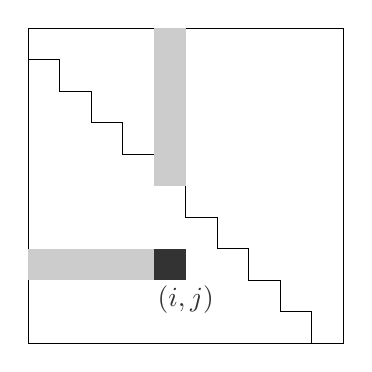
\begin{tikzpicture}[scale=0.4]
      \draw (0,0) rectangle ++ (10,10);
      \draw
      (0,9) --
      (1,9) --
      (1,8) --
      (2,8) --
      (2,7) --
      (3,7) --
      (3,6) --
      (4,6) --
      (4,5) --
      (5,5) --
      (5,4) --
      (6,4) --
      (6,3) --
      (7,3) --
      (7,2) --
      (8,2) --
      (8,1) --
      (9,1) --
      (9,0);
      \fill[black!20] (4,5) rectangle ++ (1,5);
      \fill[black!20] (0,2) rectangle ++ (4,1);
      \fill[black!80] (4,2) rectangle ++ (1,1) node[below=1em] {\((i,j)\)};
    \end{tikzpicture}
    \caption{Dependence for some \(l_{ij}\)}
  \end{subfigure}
  \begin{subfigure}{.4\linewidth}
    \centering
    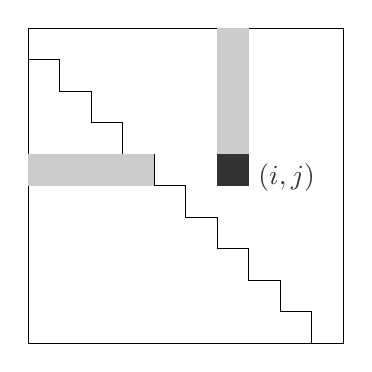
\begin{tikzpicture}[scale=0.4]
      \draw (0,0) rectangle ++ (10,10);
      \draw
      (0,9) --
      (1,9) --
      (1,8) --
      (2,8) --
      (2,7) --
      (3,7) --
      (3,6) --
      (4,6) --
      (4,5) --
      (5,5) --
      (5,4) --
      (6,4) --
      (6,3) --
      (7,3) --
      (7,2) --
      (8,2) --
      (8,1) --
      (9,1) --
      (9,0);
      \fill [black!20] (6,6) rectangle ++ (1,4);
      \fill [black!20] (0,5) rectangle ++ (4,1);
      \fill [black!80] (6,5) rectangle ++ (1,1) node[below right] {\((i,j)\)};
    \end{tikzpicture}
    \caption{Dependence for some \(u_{ij}\)}
  \end{subfigure}
  \caption[Dependence of ILU unknowns]{Formula for unknown at \((i,j)\) (dark
    square) depends on other unknowns left of \((i,j)\) in \(\matr{L}\) and
    above \((i,j)\) in \(\matr{U}\) (shaded regions).}
  \label{fig:dependence}
\end{figure}

\setcounter{figure}{0}
\setcounter{equation}{0}
\setcounter{table}{0}

\chapter{Implementation}
\label{cha:implementation}

The solver implementation combines modern C++ template programming with
numerical linear algebra techniques to support mixed-precision iterative
refinement on sparse systems. Its overall design emphasizes three guiding
principles:

\begin{description}
\item[Interface compatibility] The solver interface mimics that of Eigen’s sparse
  solvers \cite{noauthor_eigen_nodate}, ensuring easy adoption and familiarity
  for users already working within this ecosystem.
\item[Precision flexibility] All arithmetic operations are templated over precision
  types, enabling seamless use of IEEE 754 and extended floating-point formats
  in mixed-precision workflows.
\item[Modularity] Numerical kernels such as sparse matrix-vector multiplication,
  triangular solves, and vector operations are implemented in a modular
  BLAS-like layer, separating solver logic from low-level computations.
\end{description}

This chapter presents the solver interface design, the template and concept
infrastructure supporting mixed precision, extensions to an external library for
extended floating-point types, and the modular BLAS-like kernels. It then
details the key numerical algorithms implemented: the preconditioned GMRES
kernel, the fine-grained parallel ILU factorization, and the mixed-precision
iterative refinement driver that integrates them into a complete solver
pipeline.

\section{Solver Interface Design}
\label{sec:solv-inetrf-design}

A central design objective is to expose an interface resembling that of Eigen's
sparse solvers. The solver is implemented as a class template parameterized by
three precision types:
\begin{center}
  \texttt{Solver<UF, UW, UR>}
\end{center}
where the template parameters are defined as below:
\begin{description}
\item[\texttt{UF}] factorization precision, used for incomplete LU computations,
\item[\texttt{UW}] working precision, used within GMRES iterations; this is also the
  precision of the input data and the result;
\item[\texttt{UR}] residual precision, used for residual evaluation during iterative
  refinement.
\end{description}

The solver class owns a copy of the input matrix, which can be passed by value
or moved into the solver instance to avoid unnecessary copies. The interface
provides two key methods:
\begin{description}
\item[\texttt{compute()}] accepts a sparse matrix in compressed storage format and performs
  ILU factorization in precision UF;
\item[\texttt{solve()}] accepts a right-hand side vector \(\vec{b}\), executes the
  mixed-precision iterative refinement algorithm, and returns the solution
  vector \(\vec{x}\).
\end{description}

\section{C++ Templates and Mixed Precision Concepts}
\label{sec:c++-templates-mixed}

The implementation makes extensive use of C++ templates to support type-generic
arithmetic. To ensure correctness and prevent invalid instantiations, variadic
concepts are introduced.

The \texttt{FloatingPoint} concept ensures that all participating types are valid
floating-point types, including both IEEE 754 types (\texttt{float},
\texttt{double}) and extended types (\texttt{dd\_real} for quadruple precision,
\texttt{qd\_real} for octuple precision) from the QD
\cite{david_bailey_bl-highprecisionqd_2025} library.

To enforce precision hierarchies, the \texttt{PartialOrdered} concept requires a
monotonic ordering of machine epsilon values:
\begin{center}
  \(\epsilon(\texttt{UF}) \ge \epsilon(\texttt{UW}) \ge \epsilon(\texttt{UR}),\)
\end{center}
where \(\epsilon(\texttt{T}) = \texttt{std::numeric\_limits<T>::epsilon()}\) is the machine
epsilon of precision type \texttt{T}.

The \texttt{Refinable} concept combines the two concepts above and guarantees that
only valid triples (\texttt{UF}, \texttt{UW}, \texttt{UR}) can instantiate the
solver. It ensures that factorization occurs in the lowest precision and
residuals are always computed in the highest precision.

\section{Extensions to the QD Library}
\label{sec:extens-qd-libr}

The QD package provides quadruple and octuple precision through the data types
\texttt{dd\_real} and \texttt{qd\_real}, respectively. However, it lacks certain
functionality required for modern C++ interoperability. To integrate QD
seamlessly into the solver, several extensions were implemented.

\begin{description}
\item[\texttt{std::numeric\_limits} Specializations] The corresponding machine epsilon,
  maximum, minimum values were made \texttt{constexpr}, allowing QD types to
  participate in template metaprogramming and concept checks.
\item[Explicit Conversion Functions] Bidirectional explicit conversion functions
  were implemented between QD types and both built-in IEEE types
  (\texttt{float}, \texttt{double}) and fixed-width standard types
  (\texttt{std::float16\_t}, \texttt{std::float32\_t},
  \texttt{std::float64\_t}).
\item [Formatting and I/O] Implementations of \texttt{std::formatter} were added,
  enabling direct use of \texttt{std::print} and \texttt{std::format} with QD
  types.
\end{description}

\section{Modular BLAS-like Kernels}
\label{sec:modular-blas-like}

To decouple solver logic from low-level numerical kernels, all matrix and vector
operations are organized into a separate module, following the philosophy of
BLAS \cite{blackford_2002_updated}.

Each kernel is templated not only on the element type but also on the
input/output type. For example, this design allows multiplying a Compressed
Sparse Column (CSC) matrix stored in \texttt{single} precision by a dense
\texttt{double} precision vector, producing results in \texttt{double} while the
arithmetic is carried out in \texttt{dd\_real} (quadruple). Explicit
\texttt{std::static\_cast} ensures that precision hierarchies are respected.

\section{Implemented Algorithms}
\label{sec:impl-algo}

The solver integrates three core algorithmic components: a preconditioned GMRES
method, an incomplete LU factorization (ILU), and an iterative refinement (IR)
driver. Each component is fully templated in C++ and implemented with explicit
attention to mixed-precision arithmetic.

\subsection{Preconditioned GMRES}
\label{sec:preconditioned-gmres}

Algorithm \ref{algo:gmres} implements the preconditioned GMRES procedure, following
the algorithm presented in \cite{lindquist_improving_2020}. In this work, the
restarting mechanism from the original version is omitted, since the IR driver
described in Section~\ref{sec:mixed-precision-ir} naturally enforces a restart
after each refinement cycle. As a result, the GMRES kernel functions as a
building block within the mixed-precision IR pipeline, focusing solely on Krylov
subspace construction, orthogonalization, and residual minimization in the
preconditioned space.

\begin{singlespace}
  \begin{algorithm}[h]
    \caption{GMRES with left preconditioning, given matrix \(\matr{A} \in \mathbb{R}^{n \times
        n}\), right-hand side vector \(\vec{b} \in \mathbb{R}^n\), optional
      initial guess \(\vec{x}_0 \in \mathbb{R}^n\) (if not given, \(\vec{x}_0\)
      is the zero vector), preconditioner \(\matr{M}^{-1} \approx
      \matr{A}^{-1}\), tolerance \(\epsilon\), maximum number of inner
      iterations \(n_{\text{inner}}\)}
    \label{algo:gmres}
    \begin{algorithmic}[1]
      \State \(\vec{z} \gets \vec{b} - \matr{A}\vec{x}_0\) \Comment{Compute residual}
      \State \(\vec{r} \gets \matr{M}^{-1}\vec{z}\) \Comment{Apply preconditioner}
      \State \(\beta \gets \norm{\vec{r}}_2, \quad \vec{v}_1 = \vec{r} / \beta, \quad \matr{V}_1 \gets [\vec{v}_1]\) \Comment{Setup for Arnoldi process}
      \For{\(k = 1, 2, \dots, n_{\text{inner}}\)}
        \State \(\vec{w} \gets \matr{M}^{-1} \matr{A} \vec{v}_k\) \Comment{Apply preconditioner}
        \State \(\beta_1 = \norm{\vec{w}}_2\)
        \State \(\vec{w}, h_{1,k}, \dots, h_{k,k} \gets \text{MGS}(\vec{w}, \matr{V}_k)\) \Comment{Orthogonalization}
        \State \(\beta_2 = \norm{\vec{w}}_2\)
        \If{\(\beta_1 + 0.001 \times \beta_2 = \beta_1\)} \Comment{Brown/Hindmarsh condition \cite{brown_1991_krylov}}
          \State \([\vec{w}, h_{1,k}, \dots, h_{k,k}] \gets [\vec{w}, h_{1,k}, \dots, h_{k,k}] +
          \text{MGS}(\vec{w}, \matr{V}_k)\) \Comment{Reorthogonalize}
        \EndIf
        \State \(h_{k+1,k} \gets \norm{\vec{w}}_2\)
        \State \(\vec{v}_{k+1} \gets \vec{w} / h_{k+1,k}\)
        \State \(\matr{V}_{k+1} \gets [\matr{V}_k, \vec{v}_{k+1}]\) \Comment{Stack basis horizontally}
        \State Apply Givens rotation
        \State Form and store the rotation angle for the next iteration
      \EndFor
      \State \(\matr{H}_k \gets \{h_{i,j}\}_{1 \le i,j \le k}\) \Comment{Form upper
        Hessenberg matrix}
      \State Solve the least squares problem \[\vec{y}_k = \argmin_{\vec{y}\in\mathbb{R}^k} \norm{\beta e_1 - \matr{H}_k \vec{y}}_2\]
      where \(e_1 \in \mathbb{R}^{k + 1}\) is the first standard basis vector \(e_1 = [1, 0, 0, \dots, 0]\transpose\)
      \State \(\vec{x} = \vec{x} + \matr{V}_k \vec{y}_k\) \Comment{Apply correction}
      \State \Return \(\vec{x}\)

      \vspace{10pt}

      \Procedure{MGS}{$\vec{w}, \matr{V}_k$} \Comment{Modified Gram-Schmidt}
        \State \([\vec{v}_1, \dots, \vec{v}_k] \gets \matr{V}_k\)
        \For{\(i = 1, 2, \dots, k\)}
          \State \(h_{i,k} \gets \vec{w} \cdot \vec{v}_i\)
          \State \(\vec{w} \gets \vec{w} - h_{i,k} \vec{v}_i\)
        \EndFor
        \State \Return \(\vec{w}, h_{1,k}, \dots, h_{k,k}\)
      \EndProcedure
    \end{algorithmic}
  \end{algorithm}
\end{singlespace}

\subsection{Fine-Grained Parallel ILU}
\label{sec:fine-grain-parall-1}

Algorithm \ref{algo:fgpilu} follows the fine-grained parallel ILU procedure for
nonsymmetric matrices described in \cite{chow_fine-grained_2015}. Although the
input matrix is assumed to be symmetric, the nonsymmetric ILU variant was
implemented because it proved more robust during development. In particular, the
symmetric ILU formulation occasionally suffered from NaN collapse due to
square-root evaluations of the nonlinear residual when it became negative.

Despite this, the underlying matrix symmetry was still exploited when computing
the unknowns \(u_{i,j}\) and \(l_{i,j}\). Only the upper-triangular entries
\(u_{i,j}\) were explicitly iterated, while the corresponding lower-triangular
entries \(l_{i,j}\) were recovered by symmetry.

To construct the sparsity pattern with a given fill-in level, a
\texttt{std::bitset} was used to efficiently track the nonzero positions.
Because \texttt{std::bitset} requires its size to be fixed at compile time, its
length was chosen to be larger than the problem size \(n\) to ensure coverage
for all rows and columns.

\begin{singlespace}
  \begin{algorithm}[h]
    \caption{Fine-Grained Parallel ILU, given \(\matr{A} \in \mathbb{R}^{n \times n}\) with
      positive diagonal, fill-in level \(k\), maximum number of sweeps
      \(n_{\text{sweep}}\), tolerance \(\epsilon\)}
    \label{algo:fgpilu}
    \begin{algorithmic}[1]
      \State \(\matr{d_{i,i}} \gets 1 / \sqrt{|a_{i,i}|},\quad \matr{D} \gets \{d_{i,i}\}_{1
        \le i \le n}\) \Comment{Diagonal scaling factors of \(\matr{A}\)}
      \State \(\matr{A} \gets \matr{D} \matr{A} \matr{D}\)
      \Comment{Symmetrically scales \(\matr{A}\) such that \(a_{i,i} = 1\)}
      \State \(S \gets \text{sparsity pattern of } \matr{A}^{k+1}\)
      \Comment{Without computing \(\matr{A}^{k+1}\) numerically}
      \State \(\matr{U} \gets \text{upper triangular part of } \matr{A}\)
      \State \(\matr{L} \gets \text{lower triangular part of } \matr{A}
      \text{ and set } l_{ii} = 1\)
      \State \(\beta \gets \text{NLResNorm}()\) \Comment{Computes nonlinear residual norm}
      \For{\(\text{sweep} = 1, 2, \dots n_{\text{sweep}}\)}
        \For{\((i, j) \in S\) \textbf{in parallel}}
          \If{\(i > j\)}
            \State \(l_{i,j} \gets (a_{i,j} - \sum_{k=1}^{j-1} l_{i,k}u_{k,j}) / u_{j,j}\)
          \Else
            \State \(u_{i,j} \gets a_{i,j} - \sum_{k=1}^{i-1} l_{i,k}u_{k,j}\)
          \EndIf
        \EndFor
        \State \(\beta' \gets \text{NLResNorm}()\)
        \If{\(|\beta - \beta'| < \epsilon\)}
          \State break
        \EndIf
        \State \(\beta \gets \beta'\)
      \EndFor

      \vspace{10pt}

      \Procedure{NLResNorm}{}
        \State \Return
        \[
          \sum_{(i,j) \in S} \left| a_{i,j} - \sum_{k=1}^{\min(i,j)} l_{i,k}u_{k,j} \right|
        \]
      \EndProcedure
      \end{algorithmic}
  \end{algorithm}
\end{singlespace}

\subsection{Mixed-Precision IR}
\label{sec:mixed-precision-ir}

Algorithm \ref{algo:ir} outlines the IR procedure in a MP setting: after
factorization, an initial solution is obtained and iteratively refined by
solving preconditioned correction equations. Convergence is monitored through
both update and residual norms, terminating once refinements fall below machine
precision or residual stagnation is detected.

The algorithm distinguishes three precisions: the factorization precision
\(u_f\) for ILU decomposition and triangular solves, the working precision
\(u_w\) for GMRES iterations, and the residual precision \(u_r\) for recomputing
residuals. As mentioned earlier in Section~\ref{sec:c++-templates-mixed}, this
triplet \((u_f, u_w, u_r)\) is enforced through C++ templates and concepts, with
explicit conversion operators to enable exchange between types.

\begin{singlespace}
  \begin{algorithm}[h]
    \caption{GMRES-IR with ILU factorization in MP, given factorization
      precision \(u_f\), working precision \(u_w\), residual precision \(u_r\),
      maximum number of outer iterations \(n_{\text{outer}}\)}
    \label{algo:ir}
    \begin{algorithmic}[1]
      \State Perform ILU factorization of \(\matr{A}\) \Comment{at \(u_f\)}
      \State Solve \(\matr{L}\matr{U} \vec{x}_0 = \vec{b}\) \Comment{at \(u_f\)}
      \State \(\vec{r} \gets \vec{b} - \matr{A}\vec{x}_0\) \Comment{at \(u_r\)}
      \State \(\alpha \gets \infty, \quad \beta \gets \norm{\vec{r}}\)
      \For{\(i \gets 0, \dots, n_{\text{outer}} - 1\) and \(\norm{r_i} \geq \epsilon\)}
        \State \(\gamma \gets \norm{\vec{x}_i}\)
        \State Solve \((\matr{L}\matr{U})^{-1}\matr{A}\vec{d}_i =
        (\matr{L}\matr{U})^{-1}\vec{r_i}\) with preconditioned GMRES \par
        where \(\matr{M}^{-1} = (\matr{L}\matr{U})^{-1}\) \Comment{at \(u_w\)}
        \State \(\vec{x}_{i+1} = \vec{x}_i + \vec{d}_i\) \Comment{at \(u_w\)}
        \State \(\vec{r}_i \gets \vec{b} - \matr{A}\vec{x}_i\) \Comment{at \(u_r\)}
        \State \(\alpha' \gets \norm{\vec{d}_i}, \quad \beta' \gets \norm{\vec{r}_i}\)
        \If{\(\alpha' \le \gamma \times (10 \times \epsilon_{\text{mach}}(u_w))\) or \(|\beta' - \beta| < \epsilon\)}
          \State break
        \EndIf
        \State \(\alpha \gets \alpha', \quad \beta \gets \beta'\)
      \EndFor
      \State \Return \(\vec{x}_{i+1}\)
    \end{algorithmic}
  \end{algorithm}
\end{singlespace}

\setcounter{figure}{0}
\setcounter{equation}{0}
\setcounter{table}{0}

\chapter{Experiment and Evaluation}
\label{cha:exper-eval}

\section{Experimental Setup}
\label{sec:experimental-setup}

All experiments were conducted on a Intel\textsuperscript{\textregistered}
Core\textsuperscript{\texttrademark} i7-10700K CPU, with 8 physical cores (16
threads), base frequency 3.8 GHz and turbo frequency up to 4.7 GHz. The system
was equipped with 32 GB DDR4 RAM.

\section{Test Matrices}
\label{sec:test-matrices}

All test problems were drawn from the Florida Sparse Matrix Collection
\cite{davis_university_2011}, restricted to symmetric matrices.
Table~\ref{tab:test-matrices} summarizes the benchmark set, ordered by
increasing condition number.

Each matrix \(\matr{A}\) was read from a \texttt{.mtx} file using the
\texttt{fast\_matrix\_market} \cite{alistair_lugowski_fast_matrix_market_2023}
library. The right-hand side \(\vec{b}\) was constructed consistently across all
experiments from a reference solution \[\vec{x}_{\text{ref}} = (1, 1, \dots,
  1)\transpose \in \mathbb{R}^{n}, \quad \vec{b} =
  \matr{A}\vec{x}_{\text{ref}}.\] This guarantees that the exact solution is
known, enabling direct computation of both forward and backward errors.

\begin{table}[h]
  \centering
  \begin{threeparttable}
    \begin{tabular}{
      l                                              % Matrix
      S[table-format=1.1e2]                          % condest(A)
      S[table-format=1.1e1]                          % size
      S[table-format=1.1e1]                          % NNZ
      S[table-format=1.4, print-zero-exponent=false] % % NZZ
      S[table-format=1.1e3]                          % min
      S[table-format=1.1e3]                          % max
      }
      \toprule
      Matrix                     & {\texttt{condest(A)}} & {Size}  & {\texttt{nnz(A)}} & {\% NNZ} & {\texttt{min(A)}} & {\texttt{max(A)}} \\
      \midrule
      \texttt{nemeth26} \tnote{\(\dagger\)}  & 1.1e+01         & 9.5e+03 & 1.5e+06     & 2        & 1.0e-07     & 9.7e-01     \\
      \texttt{nemeth16} \tnote{\(\dagger\)}  & 3.6e+01         & 9.5e+03 & 5.9e+05     & 0.6      & 1.0e-07     & 5.2e-01     \\
      \texttt{crystm01}                & 4.2e+02         & 4.9e+03 & 1.1e+05     & 0.4      & 7.5e-15     & 1.8e-12     \\
      \texttt{Dubcova3}                & 1.1e+04         & 1.5e+05 & 3.6e+06     & 0.02     & 8.5e-22     & 2.7e+00     \\
      \texttt{bcsstk09}                & 3.1e+04         & 1.1e+03 & 1.8e+04     & 2        & 1.1e-08     & 3.9e+07     \\
      \texttt{H2O} \tnote{\(\dagger\)}       & 4.2e+04         & 6.7e+04 & 2.2e+06     & 0.05     & 6.7e-04     & 1.2e+02     \\
      \texttt{parabolic\_fem}          & 2.1e+05         & 5.3e+05 & 3.7e+06     & 0.001    & 3.2e-07     & 4.0e-01     \\
      \texttt{494\_bus}                & 3.9e+06         & 4.9e+02 & 1.7e+03     & 0.7      & 1.7e-01     & 2.0e+04     \\
      \texttt{lund\_a}                 & 5.4e+06         & 1.5e+02 & 2.4e+03     & 1e+01    & 1.2e-04     & 1.5e+08     \\
      \texttt{1138\_bus}               & 1.2e+07         & 1.1e+03 & 4.1e+03     & 0.3      & 4.8e-01     & 2.0e+04     \\
      \texttt{G3\_circuit}             & 2.2e+07         & 1.6e+06 & 7.7e+06     & 0.0003   & 3.3e-01     & 2.3e+04     \\
      \texttt{bcsstk08}                & 4.7e+07         & 1.1e+03 & 1.3e+04     & 1        & 1.8e-12     & 7.6e+10     \\
      \texttt{ecology2}                & 6.7e+07         & 1.0e+06 & 5.0e+06     & 0.0005   & 1.0e+00     & 4.0e+01     \\
      \texttt{cbuckle}                 & 8.0e+07         & 1.4e+04 & 6.8e+05     & 0.4      & 3.9e-31     & 3.7e+04     \\
      \texttt{c-66} \tnote{\(\dagger\)}      & 1.2e+08         & 5.0e+04 & 4.4e+05     & 0.02     & 2.8e-17     & 1.7e+04     \\
      \texttt{2cubes\_sphere}          & 2.9e+09         & 1.0e+05 & 1.6e+06     & 0.02     & 6.7e-15     & 2.5e+10     \\
      \texttt{bcsstk14}                & 1.3e+10         & 1.8e+03 & 6.3e+04     & 2        & 1.6e-27     & 8.9e+09     \\
      \texttt{bcsstk18}                & 6.5e+11         & 1.2e+04 & 1.5e+05     & 0.1      & 2.1e-25     & 3.1e+10     \\
      \texttt{plat362}                 & 7.1e+11         & 3.6e+02 & 5.8e+03     & 4        & 3.5e-21     & 4.6e-01     \\
      \texttt{offshore}                & 2.3e+13         & 2.6e+05 & 4.2e+06     & 0.006    & 7.2e-21     & 7.5e+14     \\
      \texttt{ct20stif}                & 2.2e+14         & 5.2e+04 & 2.6e+06     & 0.09     & 3.0e-34     & 8.9e+11     \\
      \texttt{bloweybq}                & 4.2e+18         & 1.0e+04 & 5.0e+04     & 0.05     & 2.5e-01     & 5.0e+03     \\
      \texttt{d\_pretok} \tnote{\(\dagger\)} & 5.9e+19         & 1.8e+05 & 1.6e+06     & 0.005    & 3.1e-22     & 1.6e+04     \\
      \bottomrule
    \end{tabular}
    \caption[Symmetric matrices used for experiments]{Symmetric matrices used
      for experiments. \texttt{condest(A)} is the lower bound of the 1-norm
      condition number of matrix \(\matr{A}\) computed by
      MATLAB\textsuperscript{\textregistered}.}
    \label{tab:test-matrices}
    \begin{tablenotes}
      \item[\tnote{\(\dagger\)}] Non-positive definite matrix.
    \end{tablenotes}
  \end{threeparttable}
\end{table}

\section{Mixed-Precision Notation and Configurations}
\label{sec:mixed-prec-notat}

Throughout our experiments we adopt three mixed-precision configurations,
denoted as SDD, DDD, and DDQ. S, D, and Q stand for \texttt{single},
\texttt{double}, and \texttt{quadruple}, respectively. These notations indicate
the arithmetic precision chosen for the three computational components:
factorization \((u_f)\), working \((u_w)\), and residual evaluation \((u_r)\).
Table~\ref{tab:notation} summarizes the mapping.

\begin{table}[h]
  \centering
  \begin{tabular}{lccc}
    \toprule
    Configuration & \(u_f\)    & \(u_w\) ​   & \(u_r\)       \\
    \midrule
    SDD           & \texttt{single} & \texttt{double} & \texttt{double}    \\
    DDD           & \texttt{double} & \texttt{double} & \texttt{double}    \\
    DDQ           & \texttt{double} & \texttt{double} & \texttt{quadruple} \\
    \bottomrule
  \end{tabular}
  \caption[Precision configurations for mixed-precision IR]{Notation for the three
    precision configurations tested in this work. \(u_f\) corresponds to the
    factorization precision, \(u_w\) to the GMRES working precision, and \(u_r\)
    to the residual evaluation precision.}
  \label{tab:notation}
\end{table}


\section{Residual and Error Metrics}
\label{sec:resid-error-metr}

For iterative refinement and GMRES, two measures are reported:
\begin{enumerate}
\item relative residual (backward error), given by \[\epsilon_{\text{res}} =
    \frac{\norm{\vec{b} - \matr{A} \vec{x}_k}_{\infty}}{\norm{\vec{b}}_{\infty}},\] where \(\vec{x}_k\) is the approximate solution
  after \(k\) iterations;
\item relative error (forward error), given by \[\epsilon_{\text{err}} = \frac{\norm{\vec{x}_k -
        \vec{x}_{\text{ref}}}_{\infty}}{\norm{\vec{x}_{\text{ref}}}_{\infty}}.\]
\end{enumerate}

To assess the quality of the preconditioner, the same non-linear residual norm
used in \cite{chow_fine-grained_2015} is also monitored:
\begin{equation}
  \label{eq:nonlin}
  \sum_{(i,j) \in S}
  \left| a_{i,j} - \sum_{k=1}^{\min(i,j)} l_{i,k}u_{k,j} \right|
\end{equation}

\section{Convergence of ILU}
\label{sec:convergence-ilu}

For the experiments in this section, a chunk size of 64 was used, meaning each
thread processed 64 columns per batch. This choice follows the column-to-matrix
size ratio used in \cite{chow_fine-grained_2015}.

The mixed-precision configuration employed was DDQ, i.e., factorization in
\texttt{double} precision, GMRES iterations in \texttt{double} precision, and
residual computation in \texttt{quadruple} precision. The target tolerance was set
to \num{e-15}, which is close to the machine epsilon of \texttt{double}
precision, in order to stress the iterative refinement procedure and push the
working precision toward its limits.

The outer iteration count for IR was capped at 200, while the maximum Krylov
subspace dimension for GMRES (inner iteration) was capped at 50. These bounds
were chosen to maintain consistency with the other experiments reported in this
chapter.

Table~\ref{tab:sweeps} reports the nonlinear residual norm \eqref{eq:nonlin} at
each sweep for the case of ILU(0) for matrix \texttt{bcsstk18}. The values in
parentheses indicate the total number of IR iterations performed before
convergence under the given configuration. Results are shown for varying thread
counts and number of sweeps performed.
\begin{table}[h]
  \centering
  \newrobustcmd\iter[1]{%
    (#1)
  }
  \sisetup{table-format = 1.1e4 \iter{a}}
  \begin{tabular}{
    c
    S % 1
    S % 2
    S % 3
    S % 4
    S % 5
    }
    \toprule
    Thread & \multicolumn{5}{c}{Sweeps (Iterations)}                                                                    \\
           & \text{1}          & \text{2}          & \text{3}          & \text{4}          & \text{5}          \\
    \midrule
    1      & 4.0e-13 \iter{32} & 4.0e-13 \iter{32} & 4.0e-13 \iter{32} & 4.0e-13 \iter{32} & 4.0e-13 \iter{32} \\
    2      & 4.9e+01 \iter{36} & 5.9e-01 \iter{32} & 1.5e-03 \iter{34} & 3.7e-06 \iter{32} & 1.7e-08 \iter{32} \\
    4      & 8.9e+01 \iter{38} & 1.5e+00 \iter{32} & 5.0e-02 \iter{34} & 3.9e-03 \iter{32} & 2.3e-05 \iter{32} \\
    8      & 1.3e+02 \iter{41} & 3.4e+00 \iter{34} & 1.9e-01 \iter{34} & 1.4e-02 \iter{31} & 3.9e-04 \iter{32} \\
    16     & 1.9e+02 \iter{36} & 6.0e+00 \iter{30} & 3.7e-01 \iter{32} & 3.7e-02 \iter{32} & 2.3e-03 \iter{32} \\
    \bottomrule
  \end{tabular}
  \caption[Nonlinear residual norms for matrix \texttt{bcsstk18}]{Nonlinear residual
    norms for matrix \texttt{bcsstk18} across sweeps and thread counts. Values
    in parentheses denote the number of IR iterations required for convergence.}
  \label{tab:sweeps}
\end{table}

From these results, it is evident that the number of IR iterations required for
convergence stabilizes after approximately 5 sweeps, regardless of the thread
count. Consequently, all subsequent experiments are conducted with the maximum
number of sweeps set to 5.

\section{Accuracy}
\label{sec:accuracy}

Table~\ref{tab:res-accuracy} reports the relative forward error and relative
backward error for each test matrix across three mixed-precision settings: SDD,
DDD, and DDQ. The outer iteration count was capped at 200, and the Krylov
subspace dimension for GMRES (inner iteration) was limited to 50. Level 0 ILU
preconditioning was performed with up to 5 sweeps, executed in parallel with 16
threads. A tolerance of \(\num{e-15}\) was used throughout. Entries marked with
an asterisk indicate cases where the solver did not converge in 200 iterations,
and the reported residual corresponds to the final iteration.

\begin{table}[h!]
  \centering
  \newrobustcmd\iter[1]{(#1)}
  \begin{threeparttable}
    \begin{tabular}{ l S[table-format = 1.1e3] % SDD
      S[table-format = 1.1e3] % DDD
      S[table-format = 1.1e3] % DDQ
      | S[table-format = 1.1e4 \iter{12}] % SDD
      S[table-format = 1.1e4 \iter{12}] % DDD
      S[table-format = 1.1e4 \iter{12}] % DDQ
      }
      \toprule
      Matrix \tnote{\(\dagger\)}                      & \multicolumn{3}{c}{Relative Error}            & \multicolumn{3}{c}{Relative Residual (Iterations)}                  \\
      \midrule
                                                & \text{SDD} & \text{DDD} & \text{DDQ} & \text{SDD}         & \text{DDD}         & \text{DDQ}         \\
      {\footnotesize \texttt{1138\_bus}}              & 1.7e-11    & 1.2e-11    & 2.7e-11    & 6.0e-15 \iter{41}  & 3.7e-15 \iter{45}  & 5.4e-15 \iter{40}  \\
      {\footnotesize \texttt{2cubes\_s}}              & 1.7e-15    & 2.0e-15    & 1.3e-15    & 3.2e-16 \iter{2}   & 3.2e-16 \iter{2}   & 2.1e-16 \iter{2}   \\
      {\footnotesize \texttt{494\_bus}}               & 9.8e-13    & 1.4e-12    & 1.6e-12    & 1.7e-15 \iter{14}  & 1.7e-15 \iter{14}  & 1.1e-15 \iter{13}  \\
      {\footnotesize \texttt{Dubcova3}}               & 1.5e-13    & 1.5e-13    & 1.8e-13    & 7.9e-16 \iter{8}   & 8.7e-16 \iter{8}   & 6.4e-16 \iter{8}   \\
      {\footnotesize \texttt{G3\_circu}}              & 2.3e-09    & 2.2e-09    & 3.6e-10    & 2.5e-15 \iter{50}  & 4.9e-15 \iter{50}  & 1.3e-15 \iter{54}  \\
      {\footnotesize \texttt{H2O}}                    & 1.5e-12    & 1.5e-12    & 1.2e-12    & 1.2e-15 \iter{6}   & 1.3e-15 \iter{6}   & 1.1e-15 \iter{6}   \\
      {\footnotesize \texttt{bcsstk08}}               & 1.4e-12    & 1.0e-12    & 6.7e-12    & 1.5e-15 \iter{3}   & 2.7e-15 \iter{3}   & 6.3e-16 \iter{2}   \\
      {\footnotesize \texttt{bcsstk09} \tnote{\(\ddag\)}} & 1.5e+01    & 3.4e+01    & 4.9e+01    & 2.5e+00 \iter{*}   & 2.0e+01 \iter{*}   & 2.0e+01 \iter{*}   \\
      {\footnotesize \texttt{bcsstk14}}               & 4.5e-11    & 2.8e-11    & 7.8e-12    & 4.3e-15 \iter{152} & 2.6e-15 \iter{139} & 7.7e-16 \iter{88}  \\
      {\footnotesize \texttt{bcsstk18}}               & 1.2e-10    & 1.0e-10    & 2.9e-10    & 3.9e-16 \iter{29}  & 5.9e-16 \iter{29}  & 3.0e-16 \iter{29}  \\
      {\footnotesize \texttt{bloweybq}}               & 1.8e+00    & 1.1e+00    & 1.1e+00    & 1.0e+00 \iter{2}   & 1.7e-10 \iter{*}   & 6.0e-12 \iter{83}  \\
      {\footnotesize \texttt{c-66}}                   & 1.2e-11    & 8.8e-12    & 5.6e-12    & 7.1e-16 \iter{38}  & 5.0e-16 \iter{43}  & 3.2e-16 \iter{42}  \\
      {\footnotesize \texttt{cbuckle}}                & 2.1e-12    & 1.9e-12    & 1.7e-12    & 2.6e-15 \iter{6}   & 2.2e-15 \iter{6}   & 1.7e-15 \iter{6}   \\
      {\footnotesize \texttt{crystm01}}               & 4.7e-15    & 6.2e-15    & 3.9e-15    & 6.7e-16 \iter{2}   & 6.7e-16 \iter{2}   & 4.0e-16 \iter{2}   \\
      {\footnotesize \texttt{ct20stif} \tnote{\(\ddag\)}} & 4.8e+01    & 4.6e+01    & 4.9e+01    & 3.0e-06 \iter{*}   & 2.7e-06 \iter{*}   & 3.3e-06 \iter{*}   \\
      {\footnotesize \texttt{d\_pretok}}              & 1.0e+00    & 1.0e+00    & 1.0e+00    & 5.5e-16 \iter{2}   & 5.5e-16 \iter{2}   & 5.5e-16 \iter{2}   \\
      {\footnotesize \texttt{ecology2}}               & 7.3e-01    & 7.3e-01    & 6.8e-01    & 2.6e-06 \iter{*}   & 2.3e-06 \iter{*}   & 2.3e-06 \iter{*}   \\
      {\footnotesize \texttt{lund\_a}}                & 2.3e-12    & 2.8e-13    & 8.3e-13    & 5.0e-16 \iter{2}   & 5.0e-16 \iter{2}   & 5.0e-16 \iter{2}   \\
      {\footnotesize \texttt{nemeth16}}               & 4.7e-15    & 4.8e-15    & 3.6e-15    & 8.8e-16 \iter{2}   & 8.8e-16 \iter{2}   & 6.6e-16 \iter{2}   \\
      {\footnotesize \texttt{nemeth26}}               & 2.6e-15    & 2.4e-15    & 2.2e-15    & 1.9e-15 \iter{2}   & 1.9e-15 \iter{2}   & 1.5e-15 \iter{2}   \\
      {\footnotesize \texttt{offshore}}               & 1.1e-07    & 1.1e-07    & 1.1e-07    & 4.3e-16 \iter{14}  & 4.3e-16 \iter{14}  & 3.8e-16 \iter{14}  \\
      {\footnotesize \texttt{paraboli}}               & 1.1e-11    & 1.1e-11    & 4.1e-12    & 7.4e-11 \iter{151} & 7.3e-11 \iter{115} & 5.8e-11 \iter{124} \\
      \bottomrule
    \end{tabular}
    \caption[Relative forward error and relative residual]{Relative forward
      error and relative residual for test matrices under three MP
      configurations. Rows are sorted by matrix name. Residuals are shown with
      the number of outer iterations in parentheses. Asterisks indicate cases
      where the maximum iteration limit was reached.}
    \label{tab:res-accuracy}

    \begin{tablenotes}
    \item[\(\dagger\)] Matrix identifiers have been truncated to 8 characters (see
      Table~\ref{tab:test-matrices} for full names).
    \item[\(\ddag\)] ILU factorization fluctuates and diverged.
    \end{tablenotes}
  \end{threeparttable}
\end{table}

\paragraph{Discussion}

The results in Table~\ref{tab:res-accuracy} highlight several key aspects of
accuracy behavior across the mixed-precision configurations. First, since the
reference solution used to compute the relative forward error is exact, the
relative error is consistently larger than the relative residual. This
discrepancy generally aligns with the condition number of the tested matrix.

Across most test cases, the relative error and residual are consistent across
the three MP configurations (SDD, DDD, DDQ). A slight trend of improved accuracy
is observed as higher precision is employed, though the reduction is
modest---typically within one order of magnitude. Notably, for extremely
ill-conditioned problems such as \texttt{bloweybq}, the shift from single to
double precision in factorization yields a significant improvement in relative
residual reduction.

The iteration counts further illustrate the effect of precision change. Moving
from \texttt{single} to \texttt{double} in factorization generally reduces the
number of IR iterations required for convergence. Increasing the residual
precision from \texttt{double} to \texttt{quadruple} slightly increases the
iteration count in many cases, despite achieving comparable or better accuracy.
This suggests that higher factorization generally accelerates convergence, while
higher residual precision stabilizes the residual but does not necessarily
accelerate convergence.

For the problematic cases marked with asterisks, different convergence behaviors
were observed. For \texttt{ecology2}, the residual stagnated entirely,
suggesting that increasing the Krylov subspace dimension or employing a more
robust preconditioner is necessary. For \texttt{bcsstk09} and \texttt{ct20stif},
the ILU(0) preconditioner diverged, which in turn rendered the subsequent GMRES
solve nearly unusable and resulted in large forward errors and residuals.
Interestingly, in the case of \texttt{bcsstk09}, a development run of GMRES with
the preconditioner manually removed converged to a substantially lower residual,
indicating that the breakdown originates in the ILU factorization itself rather
than in the Krylov solver. \textcite{chow_fine-grained_2015} provides a
theoretical guarantee of convergence, which stands in contrast with the
experimental failures observed here. The inconsistency suggests that the
divergence is likely due to a flaw in our current ILU implementation rather than
a fundamental limitation of the method. Multiple attempts were made to isolate
the source of the issue, but we were unable to definitively identify the cause
within the scope of this work.

\section{Timing}
\label{sec:timing}

Table~\ref{tab:timing} summarizes the factorization and solve times measured for
the same set of tests reported in Section~\ref{sec:accuracy}. Factorization time
refers to the ILU factorization, while solve time includes the cost of iterative
refinement, GMRES iterations, and residual evaluations. As before, an asterisk
denotes cases where the solver reached the maximum of 200 IR iterations, and the
timing corresponds to the capped run.

\begin{table}[h]
  \centering
  \newrobustcmd\iter[1]{#1}
  \sisetup{
    table-format = 3.3,
    print-zero-exponent = false,
    table-align-text-after = false
  }
  \begin{tabular}{
    l
    S % SDD
    S % DDD
    S % DDQ
    |
    S % SDD
    S % DDD
    S % DDQ
    }
    \toprule
    Matrix                            & \multicolumn{3}{c}{Factorization Time (s)}    & \multicolumn{3}{c}{Solve Time (s)}                          \\
    \midrule
                                      & \text{SDD} & \text{DDD} & \text{DDQ} & \text{SDD}      & \text{DDD}      & \text{DDQ}       \\
    {\footnotesize \texttt{2cubes\_sphere}} & 0.45       & 0.48       & 0.48       & 1.53            & 1.58            & 2.68             \\
    {\footnotesize \texttt{494\_bus}}       & 0.03       & 0.03       & 0.03       & 0.02            & 0.02            & 0.04             \\
    {\footnotesize \texttt{Dubcova3}}       & 0.60       & 0.65       & 0.65       & 7.28            & 7.34            & 14.61            \\
    {\footnotesize \texttt{G3\_circuit}}    & 0.41       & 0.46       & 0.46       & 470.32          & 473.81          & 600.33           \\
    {\footnotesize \texttt{H2O}}            & 0.38       & 0.46       & 0.47       & 2.83            & 3.06            & 6.48             \\
    {\footnotesize \texttt{bcsstk08}}       & 0.03       & 0.03       & 0.02       & 0.02            & 0.02            & 0.03             \\
    {\footnotesize \texttt{bcsstk09}}       & 0.04       & 0.03       & 0.02       & 0.99 \iter{*}   & 1.10 \iter{*}   & 1.88 \iter{*}    \\
    {\footnotesize \texttt{bcsstk14}}       & 0.05       & 0.05       & 0.06       & 1.45            & 1.31            & 2.09             \\
    {\footnotesize \texttt{bcsstk18}}       & 0.06       & 0.05       & 0.06       & 1.37            & 1.43            & 2.46             \\
    {\footnotesize \texttt{bloweybq}}       & 0.03       & 0.03       & 0.03       & 0.15            & 5.61 \iter{*}   & 3.64             \\
    {\footnotesize \texttt{c-66}}           & 0.07       & 0.06       & 0.05       & 7.27            & 8.63            & 13.14            \\
    {\footnotesize \texttt{cbuckle}}        & 0.21       & 0.22       & 0.22       & 0.72            & 0.73            & 1.76             \\
    {\footnotesize \texttt{crystm01}}       & 0.05       & 0.04       & 0.03       & 0.06            & 0.04            & 0.07             \\
    {\footnotesize \texttt{ct20stif}}       & 0.76       & 0.84       & 0.85       & 89.63 \iter{*}  & 93.29 \iter{*}  & 208.77 \iter{*}  \\
    {\footnotesize \texttt{d\_pretok}}      & 0.12       & 0.14       & 0.14       & 1.61            & 1.67            & 2.52             \\
    {\footnotesize \texttt{ecology2}}       & 0.25       & 0.27       & 0.28       & 892.84 \iter{*} & 911.03 \iter{*} & 1134.85 \iter{*} \\
    {\footnotesize \texttt{lund\_a}}        & 0.06       & 0.03       & 0.03       & 0.00            & 0.00            & 0.01             \\
    {\footnotesize \texttt{nemeth16}}       & 0.24       & 0.25       & 0.25       & 0.18            & 0.18            & 0.30             \\
    {\footnotesize \texttt{nemeth26}}       & 1.10       & 1.13       & 1.13       & 0.27            & 0.10            & 0.46             \\
    {\footnotesize \texttt{offshore}}       & 1.24       & 1.26       & 1.26       & 21.06           & 21.27           & 35.23            \\
    {\footnotesize \texttt{parabolic\_fem}} & 0.20       & 0.24       & 0.17       & 325.26          & 248.89          & 370.76           \\
    {\footnotesize \texttt{plat362}}        & 0.02       & 0.01       & 0.01       & 0.25            & 0.16            & 0.35             \\
    \bottomrule
  \end{tabular}
  \caption[Runtime performance for mixed-precision IR]{Factorization and solve
    times (in seconds) for test matrices under three precision configurations:
    SDD, DDD, and DDQ. Rows are sorted by matrix name. Asterisks indicate runs
    that reached the IR iteration cap of 200.}
  \label{tab:timing}
\end{table}

\paragraph{Timing Discussion}

The results in Table~\ref{tab:timing} show that, across all test matrices, the
solve phase is consistently far more expensive than the factorization phase.
This stands in contrast to the findings of \textcite{wong_exploring_2024}, where
factorization dominated the runtime. The discrepancy arises primarily from
methodological differences: while \citeauthor{wong_exploring_2024} employed a
complete LDL\textsuperscript{T} factorization, we rely on an incomplete
factorization (ILU) which has substantially less unknowns to compute. In our
implementation the factorization is additionally parallelized across multiple
threads. Since the GMRES iterations in our implementation are sequential, they
became the primary performance bottleneck, causing the solve phase to dominate
the overall runtime.

Another observation is that the time gain from performing factorization in
\texttt{single} precision versus \texttt{double} precision is minimal. This
outcome is consistent with the small contribution of factorization time relative
to the overall runtime. As solve time dominates, reducing factorization cost has
little impact on total runtime.

Finally, improving the residual computation from \texttt{double} precision to
\texttt{quadruple} precision results in a marked increase in runtime. This
slowdown arises from two sources. First, \texttt{quadruple} precision arithmetic
is intrinsically more expensive than \texttt{double} precision. Second,
higher-precision residuals demand additional GMRES iterations to converge as
observed in Section \ref{sec:accuracy}, further amplifying the computational
burden. Together, these factors explain the consistent timing increase observed
in the DDQ configuration compared to SDD and DDD.

\setcounter{figure}{0}
\setcounter{equation}{0}
\setcounter{table}{0}

\chapter{Conclusion}
\label{cha:conclusion}

This work presented the mathematical foundations, software design,
implementation, and evaluation of a mixed-precision iterative refinement solver
for large sparse linear systems, combining a fine-grained parallel ILU
factorization with a preconditioned GMRES kernel. The solver was implemented in
modern C++ with emphasis on modularity, template-based precision flexibility,
and interface compatibility with existing linear algebra ecosystems. Extensions
to the QD library were introduced to enable seamless integration of quadruple
and octuple precision types within this framework.

The experimental results demonstrated that mixed precision can improve both
accuracy and robustness, though the gains are subtler than anticipated. Moving
from single to double precision in the factorization consistently accelerated
convergence and reduced iteration counts, while raising the residual precision
from double to quadruple stabilized the refinement process but significantly
increased runtime. Overall, the runtime advantage of lower precision
factorization was modest, since solve time was consistently dominated by GMRES
iterations.

Several pathological cases highlighted limitations of the current approach. For
some matrices, the \texttt{ILU(0)} preconditioner failed to converge, producing
stagnation or divergence in the subsequent GMRES solve. Although
\textcite{chow_fine-grained_2015} established convergence guarantees for the ILU
fixed-point sweeps used in factorization, these guarantees do not extend to the
full GMRES-IR solver. The observed breakdowns therefore point to weaknesses in
the present \texttt{ILU(0)} implementation and the inherent fragility of level-0
incomplete factorizations, rather than a fundamental flaw in the iterative
refinement framework itself.

The performance profile further emphasizes this distinction. Factorization was
consistently cheaper than the solve stage, in contrast to earlier LDLT-based
implementations where factorization dominated runtime. This shift arises from
the use of parallel \texttt{ILU(0)}, which reduces factorization cost, while
GMRES iterations remained sequential and therefore became the bottleneck.

\section*{Future Directions}

Two practical extensions follow directly from the limitations observed in this
work:

\begin{description}
\item[Parallel ILU for nonsymmetric systems] Extend the current fine-grained
  parallel ILU implementation beyond symmetric/SPD matrices to fully
  nonsymmetric cases. This would require stability safeguards such as diagonal
  scaling, threshold dropping, or optional pivoting/reordering, but would
  broaden applicability to a wider range of real-world problems such as
  convection-dominated PDEs and circuit models.

\item[Stronger ILU variants] Investigate \texttt{ILU(k)} and threshold-based \texttt{ILU(T)}
  factorizations within the same parallel framework. These approaches may
  provide more robust preconditioning for ill-conditioned systems where
  \texttt{ILU(0)} failed (e.g., \texttt{ct20stif}, \texttt{ecology2}), without
  sacrificing too much efficiency.
\end{description}

\section*{Closing Remarks}

In summary, this project developed and evaluated a modern C++ solver framework
for mixed-precision iterative refinement with parallel incomplete
factorizations. The results confirm that mixed precision can enhance solver
accuracy and robustness, but also show that the benefits depend critically on
the interplay between factorization quality, preconditioner reliability, and
Krylov convergence. While the immediate performance improvements were modest,
the implementation provides insights into precision hierarchies, highlights the
importance of preconditioner design, and establishes a foundation for future
advances in mixed-precision sparse linear solvers.

\setcounter{figure}{0}
\setcounter{equation}{0}
\setcounter{table}{0}

% --------------------Appendix-------------------------
% \begin{appendix}
% 	\include{chapters_after_preface_appendix/appendix_A}
%   \setcounter{figure}{0}
%   \setcounter{equation}{0}
%   \setcounter{table}{0}

% 	\include{chapters_after_preface_appendix/appendix_B}
%   \setcounter{figure}{0}
%   \setcounter{equation}{0}
%   \setcounter{table}{0}
% \end{appendix}

% --------------------Bibliography-------------------------
% check which bibliography style your department prefers
\printbibliography{}

\label{NumDocumentPages}

\end{document}
%----------------- Document Ended ------------------


% system requirements and design needed? Briefly, not in details
% contribution of this work? Experiments
% mention of previous reports? QDLDL?
% Parallelism in literature review? No

% 2020 Precond GMRES
% Fine-grained ILU
% Mixed precision arithmetic for HPC slides


% Experiments env Sharcnet? PC is fine

% Intel 10700K

% what experiments to do?
% Kims? vs. QDLDL? vs. LUIR
% against MPIR itself, mixed precision


% include changes to the QD package


% dynamic stopping criterion for ILU
